% arXiv-ready article. Compile with pdflatex + bibtex (e.g. `latexmk -pdf main.tex`).
\documentclass[11pt]{article}

% --- Encoding & fonts ---------------------------------------------------------
\usepackage[T1]{fontenc}
\usepackage[utf8]{inputenc}
\usepackage{lmodern}
\usepackage{microtype}

% --- Page layout ----------------------------------------------------------------
\usepackage[letterpaper,margin=1in]{geometry} % 6.5in text width (see src/ai_for_rd/plotting.py)

% --- Math ---------------------------------------------------------------------
\usepackage{amsmath,amssymb,amsthm}
\usepackage{bm}

% --- Figures & tables ---------------------------------------------------------
\usepackage{graphicx}
\graphicspath{{figures/}}
\usepackage{booktabs}
\usepackage{subcaption}

% --- Citations & links (hyperref/cleveref must come last) ---------------------
\usepackage[numbers,sort&compress]{natbib}
\usepackage{xcolor}
\usepackage[colorlinks=true,linkcolor=blue!60!black,citecolor=blue!60!black,urlcolor=blue!60!black]{hyperref}
\usepackage[capitalize,noabbrev]{cleveref}

% --- Theorem environments -----------------------------------------------------
\newtheorem{theorem}{Theorem}
\newtheorem{lemma}[theorem]{Lemma}
\theoremstyle{definition}
\newtheorem{definition}[theorem]{Definition}

% --- Macros -------------------------------------------------------------------
\newcommand{\R}{\mathbb{R}}
\newcommand{\E}{\mathbb{E}}
\newcommand{\todo}[1]{\textcolor{red}{[TODO: #1]}}

% --- Title --------------------------------------------------------------------
\title{AI for R\&D: Working Title}
\author{
  Olivier Giroud\\
  Baracoda\\
  \texttt{\todo{email}}
}
\date{\today}

\begin{document}

\maketitle

\begin{abstract}
\todo{One paragraph: problem, approach, key result, why it matters.}
\end{abstract}

\section{Introduction}
\label{sec:introduction}

\todo{Motivate the problem and state the contributions.}
Recent work on large language models~\citep{vaswani2017attention} has opened new possibilities for research and development workflows.

Our contributions are:
\begin{itemize}
  \item \todo{Contribution 1.}
  \item \todo{Contribution 2.}
\end{itemize}

\section{Related Work}
\label{sec:related-work}

\todo{Position this work against prior art.}

\section{Method}
\label{sec:method}

\todo{Describe the approach.}
Given inputs $\bm{x} \in \R^d$, we minimise the expected loss
\begin{equation}
  \label{eq:objective}
  \min_{\theta} \; \E_{(\bm{x}, y)} \left[ \ell\big(f_\theta(\bm{x}), y\big) \right].
\end{equation}

\section{Experiments}
\label{sec:experiments}

\todo{Setup, datasets, baselines, results.}
\Cref{fig:example} is generated by \texttt{scripts/make\_figures.py}; \cref{tab:example} shows the table style.

\begin{figure}[t]
  \centering
  \IfFileExists{figures/example.pdf}{%
    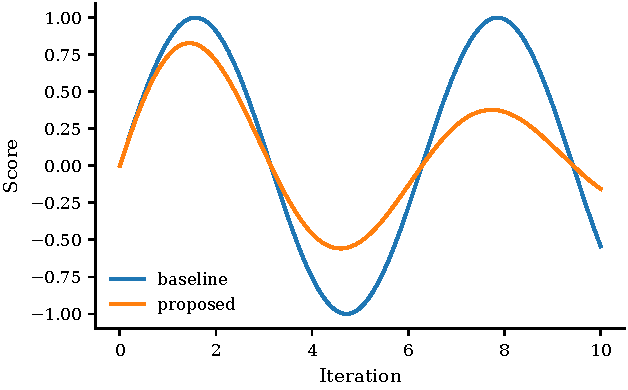
\includegraphics[width=0.7\linewidth]{example.pdf}%
  }{%
    \fbox{\parbox[c][4cm][c]{0.7\linewidth}{\centering Run \texttt{make figures}}}%
  }
  \caption{Example figure. Replace with a real result.}
  \label{fig:example}
\end{figure}

\begin{table}[t]
  \centering
  \caption{Example results table (booktabs style).}
  \label{tab:example}
  \begin{tabular}{lcc}
    \toprule
    Method   & Accuracy (\%) & Time (s) \\
    \midrule
    Baseline & 71.2          & 12.4     \\
    Ours     & \textbf{78.9} & 10.1     \\
    \bottomrule
  \end{tabular}
\end{table}

\section{Conclusion}
\label{sec:conclusion}

\todo{Summarise findings, limitations and future work.}


\bibliographystyle{plainnat}
\bibliography{references}

\appendix
\section{Additional Details}
\label{app:details}

\todo{Hyperparameters, extra results, proofs.}


\end{document}
